\section{Kafka Cluster Pi}

\begin{figure}[H]
  \centering
  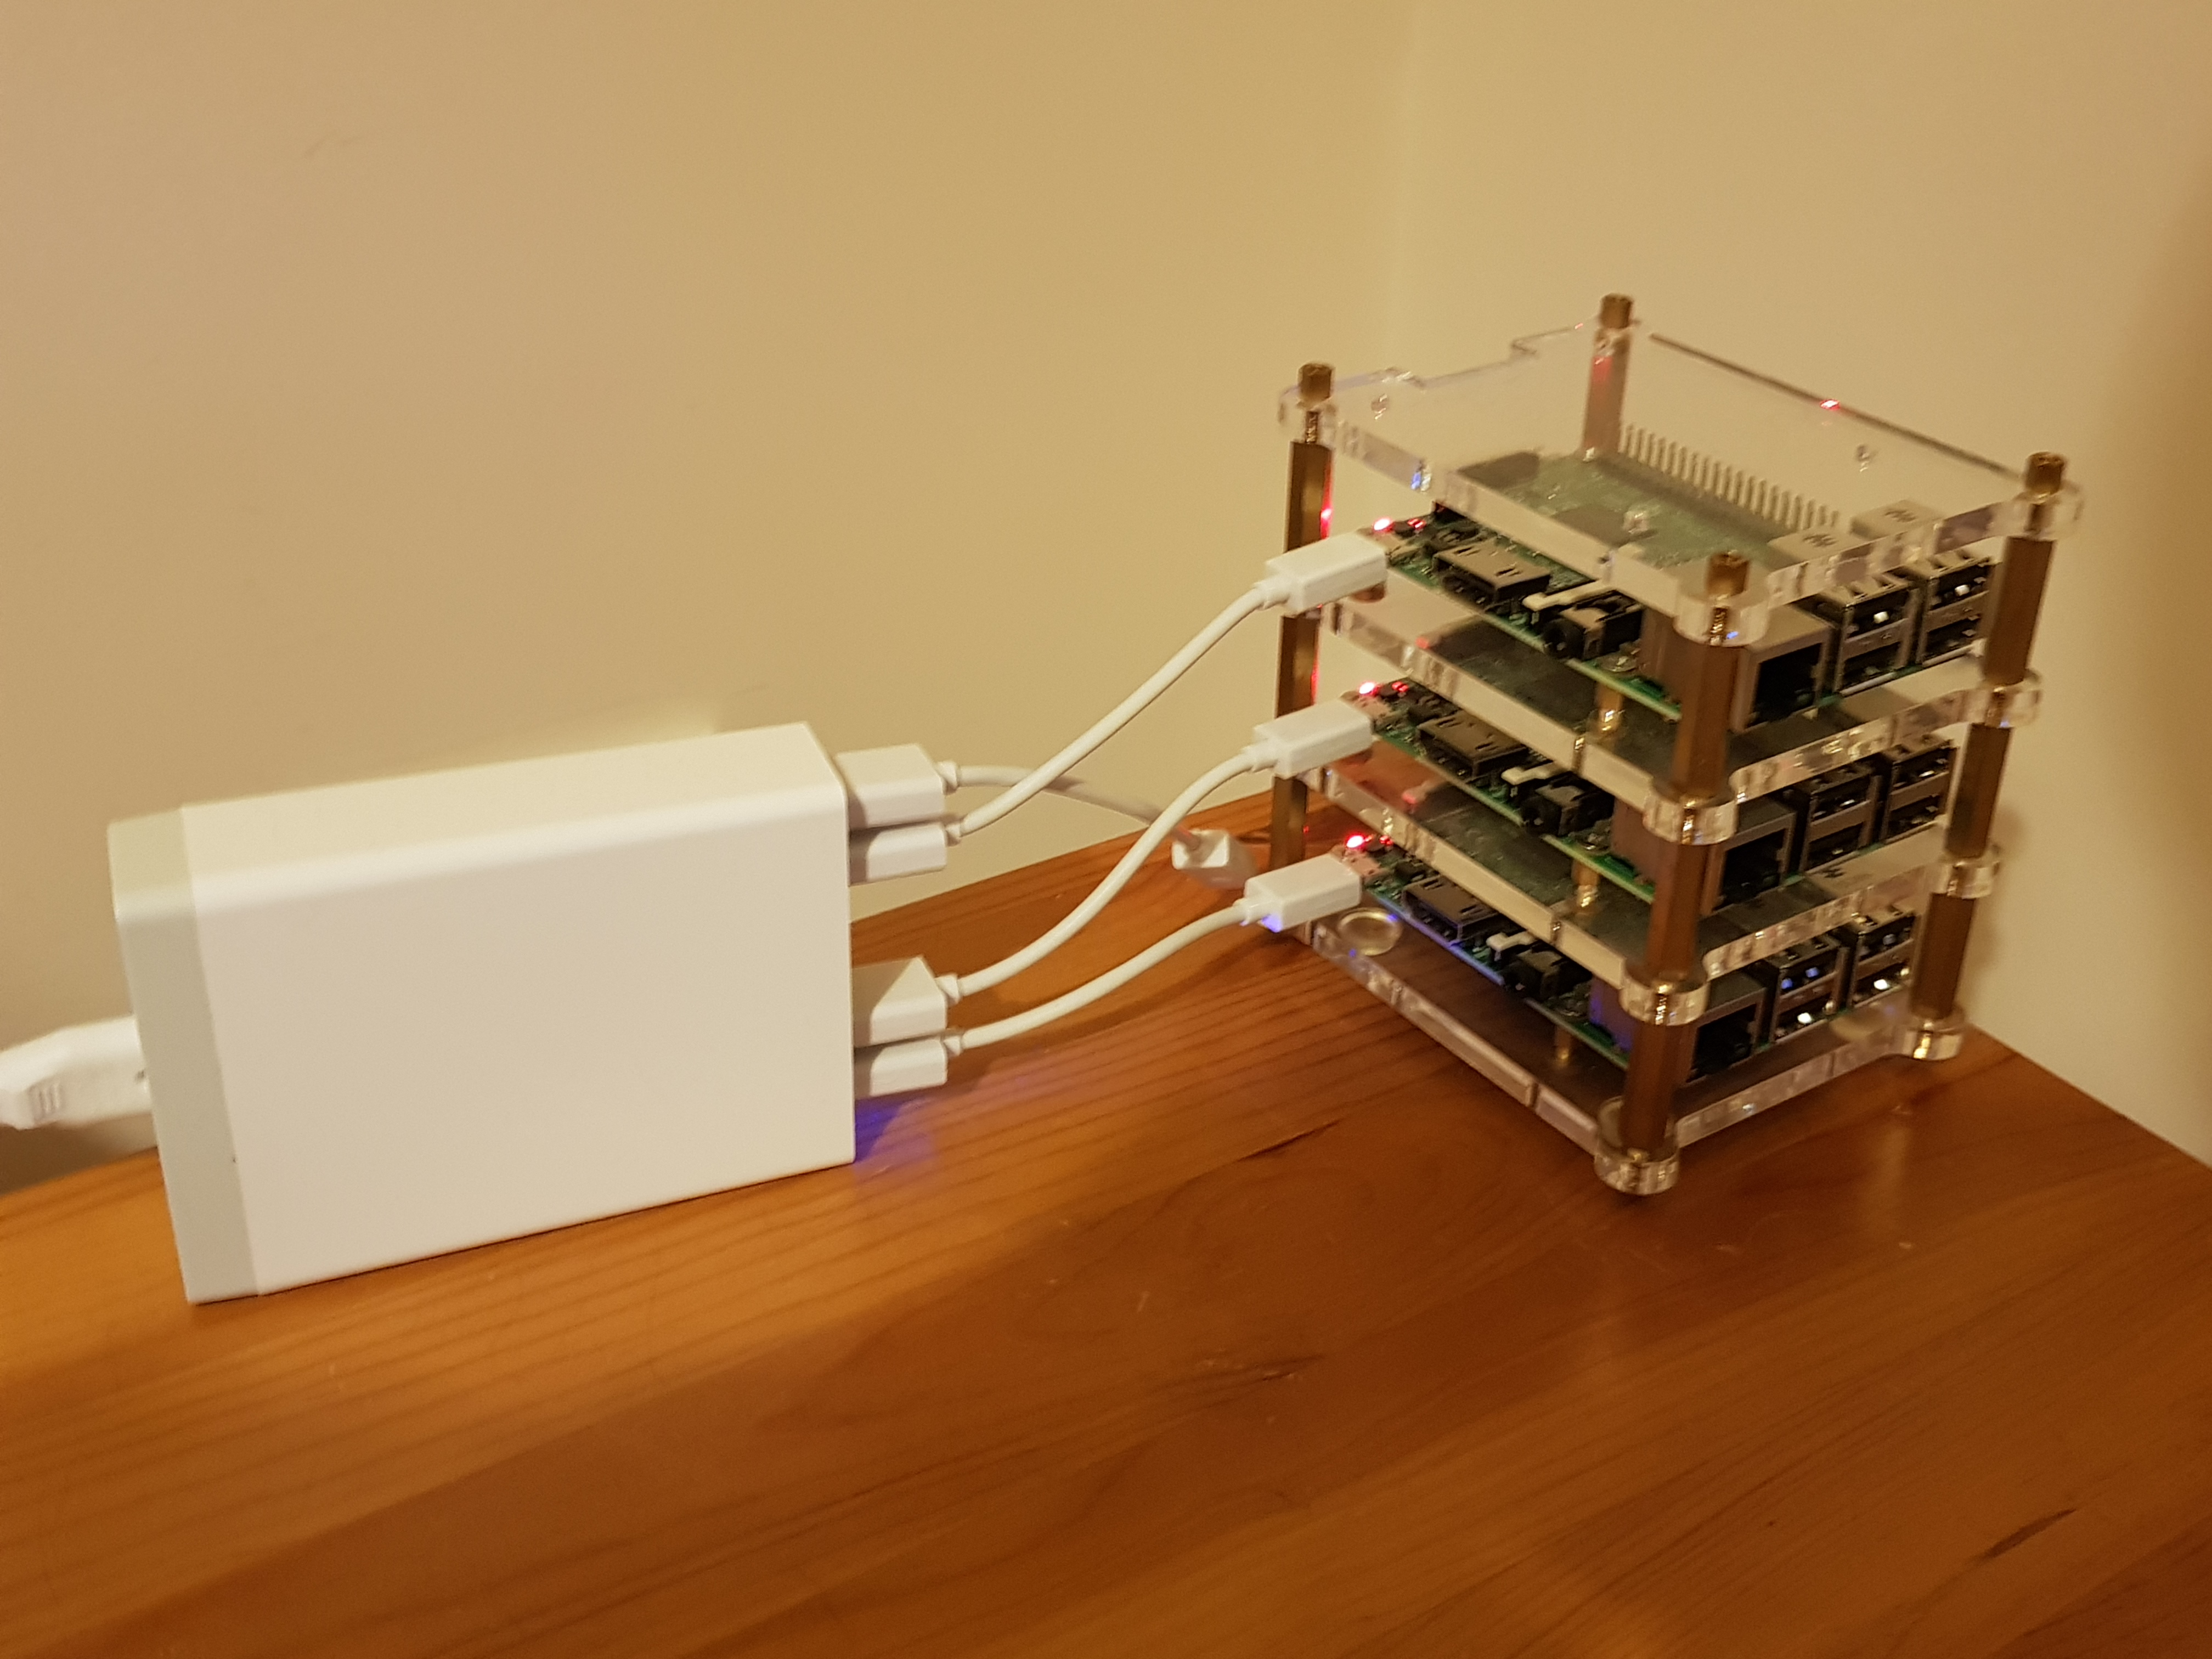
\includegraphics[scale=0.5,width=100mm]{./images/pi-cluster.jpg}
  \caption{Raspbery pi rack running Kafka and Zookeeper clusters}
  \label{fig:pi-rack}
\end{figure}

For the purposes of this document, I wanted to get a working example of a Kafka cluster working on some hardware. Rather than going for a paid solution, I went with a raspberry pi cluster instead as I had one handy. Here are the steps that I took to get a 3 node Kafka cluster running on raspberry pi. We will assume that each raspberry pi has been pre-installed with the raspbian Linux distribution and are connected to a network.

For each raspberry pi node download and unzip Kafka with the command below

\begin{minted}{bash}
  $ cd ~
  $ wget http://apache.tt.co.kr/kafka/1.1.0/kafka_2.12-1.1.0.tgz
  $ tar zxvf kafka_2.12-1.1.0.tgz
\end{minted}

Next we will need to edit the zookeeper.properties config file. Make sure to do this on each node

\begin{minted}{bash}
  $ cd kafka_2.12-1.1.0/config
  $ nano zookeeper.properties
\end{minted}

Add the following configurations to the bottom of this file

\begin{minted}{bash}
  tickTime=2000
  initLimit=10
  syncLimit=5
  clientPort=2181
  server.1=cluster-master:2888:3888
  server.2=cluster-slave-1:2888:3888
  server.3=cluster-slave-2:2888:3888
\end{minted}

Server 1, 2 and 3 are the different raspberry pi nodes. cluster-master, cluster-slave-1 and cluster-slave-2 are the assigned domain names to each of the nodes and port 2888 is the port zookeeper will run on. Next we need to make sure each server knows its own id. This can be achieved by creating a myid file. For each raspberry pi node do the following. 

\begin{minted}{bash}
  echo 1 > /tmp/zookeeper/myid
  echo 2 > /tmp/zookeeper/myid
  echo 3 > /tmp/zookeeper/myid
\end{minted}

Note only one command needs to be run on each node. For example for cluster-master we only need to run 

\begin{minted}{bash}
echo 1 > /tmp/zookeeper/myid
\end{minted}

Next we need to configure the Kafka server on each node. Run the command below

\begin{minted}{bash}
  $ nano server.properties
\end{minted}

At the bottom of the file add an entry like below

\begin{minted}{bash}
broker.id=1
port=9092
host.name=192.168.0.37
zookeeper.connect=cluster-master:2181,cluster-slave-1:2181,cluster-slave-2:2181
\end{minted}

\begin{itemize}
  \item \textbf{broker.id} is the same id as we put in the myid file
  \item \textbf{port} is the port the Kafka broker will run on
  \item \textbf{host.name} is the ip address of the raspberry pi node
  \item \textbf{zookeeper.connect} is a comma separated list of every other broker in the cluster
\end{itemize}

Next we need to edit the \textbf{kafka-server-start.sh} file. This is needed because raspberry pis have limited memory available. With this update the pi will quickly run out of memory \cite{raspberry:pi}

\begin{minted}{bash}
  $ cd ..
  $ nano bin/kafka-server-start.sh
\end{minted}

Add the following to the top of the file

\begin{minted}{bash}
  export JMX_PORT=${JMX_PORT:-9999}
  export KAFKA_HEAP_OPTS="-Xmx256M -Xms128M"
\end{minted}

If we have done all the steps mentioned above on each raspberry pi node we are now able to start our zookeeper and Kafka servers.

\begin{minted}{bash}
  $ nohup ./bin/zookeeper-server-start.sh config/zookeeper.properties & 
  $ nohup ./bin/kafka-server-start.sh config/server.properties &
\end{minted}

The first command starts zookeeper. The second command starts kafka. Both command should be executed about 30 seconds between each other to give everything a chance to come up. To test that the cluster is up and running we can create a new topic on any of the cluster nodes using the command below.

\begin{minted}{bash}
  $ /home/pi/kafka_2.12-1.1.0/bin/kafka-topics.sh --create \
  --zookeeper cluster-slave-1:2181 --replication-factor 3 \
  --partitions 5 -topic rdtest
\end{minted}